\documentclass[runningheads]{llncs}
\usepackage[english]{babel}
\usepackage[utf8x]{inputenc}
\usepackage[T1]{fontenc}

\usepackage{amsmath,amssymb}
%\usepackage[square,numbers,sort&compress]{natbib}
\usepackage{xspace}
%% Useful packages
\usepackage{graphicx}
\usepackage{pdflscape,adjustbox}
\usepackage{multirow}

\usepackage{algorithm}
\usepackage[noend]{algpseudocode}
\usepackage{booktabs} % For formal tables
\usepackage{enumitem}
\usepackage{afterpage,tabularx}
\usepackage[colorlinks=true, allcolors=blue]{hyperref}
\usepackage[square,numbers,sort]{natbib}
% Fixes for using natbib and llncs
\makeatletter
% required for natbib to have "References" printed and as section*, not chapter*
\renewcommand\bibsection%
{\section*{\refname\@mkboth{\MakeUppercase{\refname}}{\MakeUppercase{\refname}}}}
\renewcommand\@biblabel[1]{#1.}
\def\bibfont{\small}
\makeatother

% If you use the hyperref package, please uncomment the following line
% to display URLs in blue roman font according to Springer's eBook style:
\renewcommand\UrlFont{\color{blue}\rmfamily}

\newcommand{\true}{\textsc{true}}
\newcommand{\false}{\textsc{false}}
\newcommand{\NULL}{\textsc{null}}
\newcommand{\NA}{---}
\newcommand{\assign}{\ensuremath{:=}}
\newcommand{\procedure}[1]{\textsf{#1}}
\newcommand{\Inf}{\ensuremath{\infty}}
\DeclareMathOperator*{\argmax}{arg\,max}

%% Revision documents
\usepackage[dvipsnames]{xcolor}
\usepackage[normalem]{ulem}
% FIXME: \sout is not very good. It cannot handle commands within its argument.
\newcommand{\SuggestEdit}[3][red]{\textcolor{#1}{\sout{#2}}\textcolor{#1}{#3}}
\let\svthefootnote\thefootnote
\newcommand\colorfootnote[2][black]{\def\thefootnote{\color{#1}\svthefootnote}%
  \footnote{\color{#1}#2}\def\thefootnote{\color{black}\svthefootnote}}
\newcommand\RevComment[3][red]{\protect\colorfootnote[#1]{{\textbf{[#2: #3]}}}}
% Command for edits, command for commenting and color
\newcommand\newrevisor[3]{%%
  \colorlet{#1}{#3}
  \expandafter\newcommand\csname#1\endcsname[2]{\SuggestEdit[#1]{##1}{##2}}%%
  \expandafter\newcommand\csname#2\endcsname[1]{\RevComment[#1]{#2}{##1}}%%
}
\newrevisor{manuel}{MANUEL}{Purple}
\newrevisor{ekhine}{EKHINE}{red}

\hyphenation{%%% Merriam-Webster
  di-men-sion-al %%
  op-tical net-works semi-conduc-tor %%
  pher-o-mone non-dom-i-nance %%
  non-dom-i-nat-ed chro-mo-some %%
  sto-chas-tic make-span an-a-lys-ing}


\title{Mallows, Black-box combinatorial optimization, limited budget,  ???}
% Double-blind
\author{Double-blind}
% \author{Ekhiñe Irurozki\inst{1} \and Manuel López-Ibáñez\inst{2}\orcidID{0000-0001-9974-1295}}
% \institute{
%    Basque Center for Applied Mathematics\\
%    \email{eirurozki@bcamath.org}
%    \and
%    University of Málaga, Málaga, Spain\\
%    \email{manuel.lopez-ibanez@uma.es}
% }
\date{}%

\begin{document}

\maketitle

\begin{abstract}
%The abstract should briefly summarize the contents of the paper in
%150--250 words.
  Black-box combinatorial optimization problems arise in practice when the
  objective function is evaluated by means of a simulator or a real-world
  experiment. In such cases, classical techniques such as mixed-integer
  programming and local search cannot be applied. Moreover, often each solution
  evaluation is expensive in terms of time or resources, thus only a limited
  number of evaluations is possible, typically several order of magnitude
  smaller than in white-box optimization problems. In the continuous case,
  Bayesian optimization, in particular using Gaussian processes, has proven
  very effective under these conditions. Much less research is available in the
  combinatorial case. In this paper, we propose and analyze an
  estimation-of-distribution (EDA) algorithm based on a Mallows probabilistic
  model and compare it with CEGO, a Bayesian optimization algorithm for
  combinatorial optimization. Experimental results show that the Bayesian
  algorithm is able to obtain very good solutions with very few evaluations,
  however, at a significant computational cost, whereas the proposed EDA
  outperforms CEGO when the number of solutions evaluated approaches 400, and
  it is significantly faster. These results suggest that the combination of
  Bayesian optimization and a Mallows-based EDA may be an interesting direction
  for future research.
\textcolor{red}{16 pages max, deadline: 1 November 2020}
\keywords{Combinatorial optimization \and Bayesian optimization \and Expensive black-box optimization \and Estimation of distribution algorithms}
\end{abstract}

\section{Introduction}

Motivation: Manuel

In many practical optimization problems, the objective function is not
explicitly available and solutions are evaluated by means of expensive
prediction models, simulations or physical experiments. When decision variables
are continuous, the use of Bayesian surrogate-models, e.g., Gaussian processes,
in optimization has become
widespread~\citep{JonSchWel98go,ForKea2009surrogate}. Motivated by this
success, there have been attempts at adapting such Bayesian optimization
algorithms to the combinatorial case, a notable example being Combinatorial
Efficient Global Optimization
(CEGO)~\citep{ZaeStoBar2014:ppsn,ZaeStoFriFisNauBar2014}. However, the
ruggedness of combinatorial landscapes, which makes local search particularly
effective in the white-box context, lessens the effectiveness of global
surrogate models~\citep{EriPeaGar2019scalable}. Moreover, surrogate models are
expensive to train and optimize. The additional time required by the Bayesian
optimizer may impose a significant overhead in computation time, specially if
computation time of each function evaluation is measured in ``few'' minutes or
hours rather than days and when ``expensive'' refers to resources or economical
cost rather than wall-clock time. \citet{PerLopStu2015si} recently showed that
ant colony optimization (ACO)~\citep{DorStu2004:book} is competitive with CEGO
on a black-box version of the travelling salesman problem under a budget of
$1\,000$ function evaluations. ACO basically builds a probability distribution
model from which solutions are sampled with a bias towards the best solutions
evaluated so far. As such, ACO may be considered a type of
estimation-of-distribution algorithm (EDA) for combinatorial optimization. On
the other hand, $1\,000$ evaluations is a relatively large budget for CEGO and
ACO was not designed for such short budgets.

In this work, we propose and analyze uMM, an EDA specifically designed for
black-box combinatorial optimization under a limited budget. The proposed uMM 
\EKHINE{yo no diria que es un EDA porque  no hay generaciones de muestras que compiten }
\ldots\MANUEL{what is the inspiration}
\EKHINE{we propose a probabilistic algrithm that (like cego?) (1) iteratively adds solutions to the sample and (2) fits a surrogate model for every new sample obtained. However,  different fom cego, our surrogate model is an estimation of the predicted fitness function at each point. CEGO controls the  intensification-explotation balance with the expected improvement??? We mimic the intensification-explotation balance by automatically controllong the variance of our surrogate model.}

% minimize the uncertainty in the final solutions or

Related work: Ekhine

Our contribution: Ekhine
\begin{itemize}
\item 
\end{itemize}


\citep{LopDubPerStuBir2016irace}

<<<<<<< HEAD
\section{Background}\label{sec:backgroud}

Permutations are defined as bijections of the set $[n]$ integer onto itself. The set of all permutations of $n$ items is denoted as $S_n$ and has cardinality $n!$. We denote permutations with Greek letters with exception of the identity permutation denoted as $e=1, 2, 3, \ldots,n$. We denote the composition of $\sigma$ and $\pi$ as $\sigma\pi$ and the inverse of $\sigma$ as $\sigma^{-1}$, for which the relation $\sigma\sigma_{-1}=e$ always holds. 

Distributions over permutations~\cite{critchlow91} are functions that assign a probability value to each of the permutations in $S_n$, $p(\sigma)\in[0,1]$. One of the most popular distributions is the Mallows Model (MM), which is considered as an analogous to the Gaussian distribution for permutations. The MM defines the probability of each permutation $\sigma$ as follows:

\begin{equation}
p(\sigma)=\frac{\exp(-\theta d(\sigma, \sigma_0))}{\psi}
\end{equation}
with two parameters, $\theta$ and $\sigma_0$, Permutation $\sigma_0$ a reference permutation that has the largest probability value, i.e., the mode of the distribution. The probability of every permutation $\sigma\in S_n$ decays exponentially as its distance $d(\sigma,\sigma_0)$ increases, and $\theta$, the dispersion parameter controls this decay. The distance $d(\sigma,\sigma_0)$ is the Kendall's-$\tau$ distance. The normalization constant $\psi$ can be easily computed for the Kendall's-$\tau$ distance as well as for the Hamming, Cayley and Ulam distance~\cite{Irurozki2016b}. 

The learning process is divide in two stages: first, we estimate the central permutation of the distribution, $\hat\sigma_0$ and, second, compute the dispersion parameter, $\hat\theta$~\cite{Irurozki2016b}. 

The exact maximum likelihood estimator (MLE) for $\sigma_0$ is given by the well-known Kemeny ranking~\cite{Dwork:2001:RAM:371920.372165}. Unfortunately,  obteinig such ranking is NP-hard~\cite{Dwork:2001:RAM:371920.372165}. An alternative to the Kemeny ranking is the Borda ranking~\cite{Ali2011}, which has several advantages. First, Borda requires polynomial computational time. Second, Borda as an estimator for the MM is guarantied to obtain high quality parameters~\cite{Caragiannis2013}. Finally, in a general optimization perspective, Borda error is bounded~\cite{Coppersmith:2010}.

The Borda ranking of sample $S$ is computed as follows: first, for each item $i$ compute its Borda score $B(i) =  \sum_{t\in S}  \sigma_t(i)$. Then, assign rank 1 to the item with the smallest Borda score, rank 2 to the item with the second smallest score and so on, i.e., order the items by Borda score increasingly. 

\subsection{Unbalanced Borda}\label{sec:uborda}
In these lines we introduce the core for our probabilisitc algorithm, the uBorda algorithm. Following the convention of the community, the ranking returned by the uBorda algorithm will be denoted uBorda ranking. The uBorda algorithm is a recent generalization of Borda~\cite{}. In uBorda, the score of item $i$ is defined as follows:

\begin{equation}
\begin{split}
B(i) =  \sum_{t\in S}  w(\sigma_t) \sigma_t(i),
\end{split}
\label{eq:uborda_score}
\end{equation}
and, the same as Borda, orders the items increasingly by their score. 

Intuitively, the uBorda ranking of sample $S$ is equivalent to the Borda ranking of $S'$, being $S'$ an extension of $S$ where each each $\sigma\in S$ has been replicated proportionally to its weight $w(\sigma)$. In this paper, we would like to replicate each permutation $\sigma$ a number of times that is proportional to $f(\sigma)$. Therefore, we will use $w(\sigma)=\rho^{f(\sigma)}$ for a $\rho\in(0,1)$. 

By setting $\rho=1$ the original Borda is recovered. However, for $\rho<1$ uBorda ranking will be closer to the rankings in $S$ with smaller value of $f(\sigma)$. Interestingly, Borda is computed in polynomial time. Clearly, the choice of the weight depends on the relevant property of a ranking in a particular domain. For example, it has been shown to have nice theoretical properties for the online estimation of the parameters of a sample with concept drift. 
=======
\newcommand{\Prob}{\ensuremath{p}}
\newcommand{\minit}{\ensuremath{m_\text{ini}}\xspace}
\newcommand{\FEmax}{\ensuremath{\textit{FE}_{\max}}}
>>>>>>> a940b6e14db49ed2a1764c0475f43374e74b6f31


\section{Background}\label{sec:backgroud}



\subsection{Black-box Combinatorial Optimization under a limited budget}

Permutations are defined as bijections of the set $[n]$ \manuel{integer}{of integers} onto itself. The set of all permutations of $n$ items is denoted as $S_n$ and has cardinality $n!$. We denote permutations with Greek letters with exception of the identity permutation denoted as $e=\manuel{}{(}1, 2, 3, \dotsc,n\manuel{}{)}$. We denote the composition of $\sigma$ and $\pi$ as $\sigma\pi$ and the inverse of $\sigma$ as $\sigma^{-1}$, for which the relation $\sigma\sigma^{-1}=e$ always holds. 

Let us assume a black-box ``fitness'' function that must be minimized over a
space of permutations $f\colon S_n \to \mathbb{R}$. Being black-box means that
we can evaluate any candidate permutation $\sigma \in S_n$ to obtain
$f(\sigma)$, however, we do not know anything else about the form of
$f$. Moreover, the evaluation of $f$ is expensive in computation time or
resources and, thus, limits the budget of candidate permutations that we can
evaluate to a relatively low number. Here, we will study budgets lower than
400. Such expensive black-box combinatorial problems arise in
manufacturing~\citep{FerAlvDiaIglEna2014ants}, where the evaluation function
may involve expensive simulations for which no closed-form mathematical
description is available.


\subsection{CEGO}

Combinatorial Efficient Global Optimization
(CEGO)~\citep{ZaeStoFriFisNauBar2014} is an extension of the well-known EGO
method~\citep{JonSchWel98go} to unconstrained black-box combinatorial
optimization problems. In EGO, Gaussian process models are used as a surrogate
of the landscape of the expensive original problem. An optimization method
searches for solutions in the surrogate model by optimizing the expected
improvement criterion, which balances the expected mean and variance of the
chosen solution. Once a solution is chosen, it is evaluated on the actual
objective function and the result is used to update the surrogate-model,
hopefully increasing its predictive power.

CEGO replaces the Euclidean distance measure, used by the surrogate model in
EGO, with a distance measure appropriate to combinatorial
landscapes~\citep{ZaeStoBar2014:ppsn}, such as the Kendall distance for
permutations~\citep{?}. In CEGO, the surrogate model is explored by a GA with
crossover and mutation operators appropriate for the particular combinatorial
problem. The original paper notes that coupling the GA with local search does
not improve the results significantly since the model is anyway an inexact
estimation of the original objective
function~\citep[p.~875]{ZaeStoFriFisNauBar2014}.

What else do we need to say?

\subsection{Distributions over permutations}
Distributions over permutations~\cite{critchlow91} are functions that assign a probability value  $\Prob(\sigma)\in[0,1]$ to each permutation $\sigma \in S_n$. One of the most popular distributions is the Mallows Model (MM), which is considered as an analogous to the Gaussian distribution for permutations. The MM defines the probability of each permutation $\sigma$ as follows:
%
\begin{equation}
\Prob(\sigma)=\frac{\exp(-\theta d(\sigma, \sigma_0))}{\psi}
\end{equation}
%
with two parameters, $\theta$ and $\sigma_0$, \manuel{Permutation $\sigma_0$ a reference}{where $\sigma_0$ is the}  permutation that has the largest probability value, i.e., the mode of the distribution. The probability of every permutation $\sigma\in S_n$ decays exponentially as its distance $d(\sigma,\sigma_0)$ increases, and the dispersion parameter $\theta$  controls this decay. The distance $d(\sigma,\sigma_0)$ is the Kendall's $\tau$ distance.\MANUEL{Can we define briefly Kendall's tau?} The normalization constant $\psi$ can be easily computed for the Kendall's $\tau$ distance as well as for the Hamming, Cayley and Ulam distances~\cite{IruCalLoz2016permallows}. 

The learning process\MANUEL{what learning process?} is divide in two stages: first, we estimate the central permutation of the distribution, $\hat{\sigma}_0$ and, second, \manuel{compute}{estimate} the dispersion parameter, $\hat\theta$~\cite{IruCalLoz2016permallows}. 

The exact maximum likelihood estimator (MLE) for $\sigma_0$\MANUEL{for $\sigma_0$ o for $\hat{\sigma}_0$?} is given by the well-known Kemeny ranking~\cite{DwoKumNao2001rank}. Unfortunately,  obtaining such ranking is NP-hard~\cite{DwoKumNao2001rank}. An alternative to the Kemeny ranking is the Borda ranking~\cite{AliMei2011kemeny}, which has several advantages: (i) it requires polynomial computational time; (ii) it  guaranties  high quality parameters as an estimator for the MM~\cite{CarProSha2013votes}; and (iii) in a general optimization perspective, Borda error is bounded~\cite{CopFleRur2010ordering}.

The Borda ranking of \manuel{sample $S$}{a sample of permutations $S \subset S_n$} is computed as follows. First, for each item $i$ compute its Borda score $B(i) =  \sum_{t\in S}  \sigma_t(i)$. Then, assign rank 1 to the item with the smallest Borda score, rank 2 to the item with the second smallest score and so on, i.e., order the items by Borda score increasingly.\MANUEL{sorry, I don't follow here, what is an item? What does $\sigma_t(i)$ means?}

\subsection{Unbalanced Borda}\label{sec:uborda}
We introduce now the core for our probabilistic algorithm, the uBorda algorithm. Following the convention of the community, the ranking returned by the uBorda algorithm will be denoted uBorda ranking. The uBorda algorithm is a recent generalization of Borda~\cite{???}.\MANUEL{This paper is missing} In uBorda, the score of item $i$ is defined as follows:
%
\begin{equation}
\begin{split}
B(i) =  \sum_{t\in S}  w(\sigma_t) \sigma_t(i),
\end{split}
\label{eq:uborda_score}
\end{equation}
%
and, the same as Borda, orders the items increasingly by their score.\MANUEL{what is $w()$?}

Intuitively, the uBorda ranking of sample $S$\MANUEL{What is $S$?} is equivalent to the Borda ranking of $S'$, being $S'$ an extension of $S$ where each each $\sigma\in S$ has been replicated proportionally to its weight $w(\sigma)$.\MANUEL{so $w$ is a weight function from $w\colon S_n \to \mathbb{R}$?} In this paper, we would like to replicate each permutation $\sigma$ a number of times that is proportional to $f(\sigma)$.\MANUEL{We have not defined $f$ but I guess it is fintess, however, we minimize $f$, so how you handle that? I guess we need to define the black-box optimization problem earlier than here} Therefore, we will use $w(\sigma)=\rho^{f(\sigma)}$ for a $\rho\in(0,1)$.
%
By setting $\rho=1$ the original Borda is recovered. However, for $\rho<1$ uBorda ranking will be closer to the rankings in $S$ with smaller value of $f(\sigma)$.\MANUEL{by ``with smaller value'' do you mean ranking for increasing values of $f(\sigma)$?} Interestingly, Borda is computed in polynomial time. Clearly, the choice of the weight\MANUEL{by weight you mean $\rho$?} depends on the relevant property of a ranking in a particular domain. For example, it has been shown to have nice theoretical properties for the online estimation of the parameters of a sample with concept drift.\MANUEL{where? Do we miss a citation here?} 



\section{Unbalanced Mallows model: probabilistic BB optimization}

LOP: Ekhine

Quizás luego: PFSP y QAP


cosas de intro : 
This new methodology relies on the assumption that the fitness landscatpe is correlated with a distribution over the same space. 
Previous paper have confirmed this point
For this case study, we show that this case for the Mallows model under the Kendall distance and 



In this section, we introduce our main contribution: We present a new methodology for the optimization of black box functions with a minimal number of queries. This methodology is a probabilistic, population-based algorithm. 

Essentially, the algorithm  considers a sample of permutations along with the fitness of each of them. It is an iterative process in which the number of iterations is fixed. 
Then, at each iteration, UMM (i) estimates a surrogate distribution of the fitness function and (ii) proposes a good fitted individual. \MANUEL{Hay un poco de duplicación entre lo anterior y lo siguiente, no?}


In this section we describe our main contribution: a novel algorithm for the optimization of a black box function over permutation spaces. This algorithm is called Unbalanced Mallows model (UMM) since it a probabilistic method based on a well-known probability distribution for permutations: the Mallows model.\MANUEL{this sounds as if this was the first time you talk about MM, but you already described it above, no? } 

\begin{algorithm}[t]
 \caption{UMM: Unbalanced Mallows Model for Black-Box Optimization}
 \label{alg:umm}
  \begin{algorithmic}[1]
    \Require $n$: ?, $m$: budget of evaluations,\newline $S$: initial permutations, $F$: their fitness values
    \For{$i \assign 1$ \textbf{to} $m$ \text{evaluations}}
    \State $\hat\sigma_0 \assign \text{uBorda}(S, F,\rho)$
    \State linear decrease on $\theta$
    \State $\sigma \assign$ sample from a $MM(\hat\sigma_0, \theta)$
    \State $S \assign S \cup \{\sigma\}$
    \State $F \assign F \cup \{f(\sigma)\}$
    \EndFor 
    \State \Return $S$, $F$
  \end{algorithmic}
\end{algorithm}


As shown in Algorithm~\ref{alg:umm}, UMM  starts with a \emph{small} sample of $m'$ permutations,\MANUEL{but the algorithm requires $m$, no $m'$?} $S=\{\sigma_1, \dotsc,  \sigma_{m'}\}$ that are randomly generated. UMM also keeps the function evaluation of each solution, $F=\{f(\sigma_1), \ldots, f(\sigma_{m'})\}$.  Then, for $m$ iterations\EKHINE{esto es exactamente así o es $m-m'$?}, UMM generates a random, promising candidate solution $\sigma$ from a probabilistic model and includes it in the sample $S$ while $f(\sigma)$ is included in $F$. At each iteration, the internal probabilistic model is updated. 


The probabilistic model is a MM that assigns higher probability values to the permutations in which the fitness value is known or expected to be minimized. The main contribution of our approach is that the distribution does not represent the current sample $S$ considered by the algorithm but instead, represents a variation of it. This variation is based on the uBorda algorithm described in Section~\ref{sec:uBorda} and is abstractly equivalent to replicating in the sample the permutations \manuel{inversely proportionally}{a number of times inversely proportional} to their fitness values, i.e., there will be many copies of the good solutions and few of the bad ones. One key property of UMM is the computational complexity of working with the original sample and the transformed sample is the same, i.e., polynomial. However, the question of how many times should we replicate each permutation in the sample? UMM includes a parameter $\rho$ that controls this point and will be detailed in Section~\ref{sec:learning}.\MANUEL{is this $\rho$ the same we explained earlier?}

At each iteration of the algorithm the following steps take place: (1) randomly
generate a permutation distributed according to the internal model and include
it in the sample and (2) evaluate the new permutation and update the
probabilistic model. These steps correspond to two statistical operations: (1)
sample a probability distribution and (2) learn a probability distribution of
the transformation of the sample. Both are describe in the subsequent sections.

\subsubsection{Learning step.}\label{sec:learning}
As shown in Section~\ref{sec:backgroud}, MM can be approximately learnt in two steps (1) estimating the location parameter $\sigma_0$ and (2) computing the scale parameter $\theta$. Since the scale parameter is set automatically,\MANUEL{How is it set automatically?} we focus on estimating $\sigma_0$.
%In order to minimize the number of permutations in the sample (and consequently the number of function evaluations) our proposed UMM learns the distribution of a transformation of the sample rather than the sample. This transformation consists on replicating the best fitted permutations. However, this is done abstractly: 
The location parameter of a MM is usually approximated with the Borda algorithm. Since we are interested on biasing the model towards the regions of the space where the fitness function is smaller, we would like to replicate the permutations a number of times that is inversely proportionally to their fitness values.
We can simulate the replication of the best fitted individuals by using uBorda, described in Section~\ref{sec:uborda} and setting $w(\sigma)=\rho^{f(\sigma)}$. This generalization requires setting a value for parameter $\rho$. We show how to choose this value in the experimental section.\MANUEL{I thought we select it automatically now?} 


\subsubsection{Sampling step.}
Sampling can be done efficiently~\cite{IruCalLoz2016permallows} given the parameters that describe the model, i.e., $\sigma_0$ and $\theta$. Given these two parameters, sampling a MM has been studied in \cite{Collas}\cite{IruCalLoz2016permallows}\cite{Regenwetter2004}\MANUEL{You call this Regenwetter, but the author is Doignon?} where the computational complexities are $O(n\log n)$ and $O(n^2)$.
%
At each iteration of UMM, $\sigma_0$ is the permutation obtained as a solution in the previous learning step. The scale $\theta$, in the other hand, is set automatically by the algorithm to control the diversification and intensification trade off: At the first iteration it is set so that the expected distance equals  ${n\choose 4}$ (half of the distance of the uniform distribution), and then it linearly decrease until the last iteration where the expected distance equals 1. Similar approaches consisting of changing the variance to control the exploration-explotation tradeoff have been taken in different contexts~\cite{arza2019approaching}.\MANUEL{there is something wrong with this reference}
%
This setting reflects the fact that, despite believing that the best global optimum at each iteration is $\sigma_0$, the uncertainty at the first stages of the algorithm is high and\MANUEL{and?}



\subsection{Comparison to standard probabilistic optimization approaches.}
UMM is a population based algorithm. There exists a wide body of research on population based probabilistic algorithms, where most prominent examples are Estimation of Distribution Algorithms (EDAs). Our approach drastically differs from EDAs since EDAs assume that function evaluations are cheap and they can do many of them. On the contrary, UMM minimizes the number of function evaluations. Moreover, UMM does not rely on an evolving sequence of samples (called generations in evolutionary approaches). Instead, UMM considers a single sample of permutations during the whole execution that is increased iteratively, with one permutation each iteration.\MANUEL{I would suggest to move this subsection to the intro, is that OK?} 
\ekhine{bayesian optim}{ff}
\EKHINE{subir a arxiv uBorda}








\section{Experimental setup}

We use the implementation of GECO provided by the
authors\footnote{\url{https://cran.r-project.org/package=CEGO}}. Following the
authors of CEGO~\citep{ZaeStoFriFisNauBar2014,ZaeStoBar2014:ppsn}, we use and
the GA that optimizes the surrogate models uses a population size of 20,
crossover rate of 0.5, mutation rate of 1, tournament selection of size 2 and
probability of 0.9, interchange mutation (i.e., exchanging two randomly
selected elements of the permutation) and cycle crossover for permutations. The
authors of CEGO used a budget of $10^4$ evaluations using the surrogate-model
for each run of the GA, however, with such setting, each run of CEGO requires
more than a week of computation time, which was infeasible for us, hence, we
set a value of \textcolor{red}{$10^3$}.

Although it is never stated in the original paper, the implementation of CEGO
generates a set of initial solutions of size $\minit=10$ by means of a
max-min-distance sequential design: new solutions are added to the set
sequentially by maximizing the minimum distance to solutions already in the
set. These initial solutions are then evaluated on the actual objective
function and the result is used to build the initial surrogate
model.% \citet{ZaeStoBar2014:ppsn} uses 10

The CPU time required for a single run of CEGO using these settings is larger
than a week.  For simplicity, we use Kendall Tau distance~\citep{?} in all
experiments\MANUEL{\citet{ZaeStoBar2014:ppsn} claims this is called Swap
  distance, could you double-check?}. Nevertheless,
\citet{ZaeStoFriFisNauBar2014} points out that CEGO performs best on the QAP
when using Hamming distance. We plan to extend our analysis of uMM to other
distance measures and to the dynamic selection of distance
measures~\citep{ZaeStoBar2014:ppsn}.

In all experiments, we consider a maximum budget of $\FEmax=400$ evaluations of
the actual objective function. In a white-box context, state-of-the-art
algorithms for the problems considered here typically evaluate
\textcolor{red}{hundreds? thousands?} of solutions, thus, the budget considered
here for the black-box context is extremely limited.

We implemented UMM in Python 3. The parameter settings that we use are...

Complete this with details of uMM: MANUEL

\manuel{Computing system details: MANUEL}{%
  All experiments were run on Intel Xeon ``Ivybridge'' E5-2650v2 CPUs at 2.60\,GHz, 64\,GB RAM
  running CentOS Linux release 7.4.1708 (Core).  }


Describir como se generan las intancias de LOP: Ekhine

Describir las instancias: Ekhine

For the LOP, we generated synthetic instances of size $n=20$, $m=200$, $\phi\in\{0.5,0.7,0.9\}$\MANUEL{what is $m$?}

In the case of the QAP and PFSP, we consider the same instances as
\citet{ZaeStoFriFisNauBar2014,ZaeStoBar2014:ppsn}, i.e.,
\texttt{nug12},\texttt{nug30},\texttt{tho30} and \texttt{kra32} for the QAP,
with $n$ equal to the number in the instance name, and \texttt{reC05},
\texttt{reC13}, \texttt{reC19}, \texttt{reC31} for the PFSP, with
$n \in \{20, 20, 30, 50\}$, respectively.

\section{Experimental analysis}


To better understand the behaviour of the algorithms, we record the fitness of
the solution evaluated at each step of each run and we average those values
over 10 runs with different random seeds on the same problem instance.  As an example, each line in Fig.~\ref{fig:lop_synth} 
shows the mean fitness of the solutions evaluated by either uMM or CEGO on one synthetic LOP
instance. The shaded area shows one standard deviation around the
mean. Ideally, each new evaluation will monotonically improve in fitness, since each solution evaluated helps to refine the model and leads to a
better solution being evaluated in the next step.  However, it is often the case that  \EKHINE{yo diría solo que lo esperable es que baje monotonically, sin entrar a valorar un ejemplo concreto}\MANUEL{Así está mejor? Quiero llamar la atención porque normalmente se muestra la evolución de la mejor solución encontrada pero nosotros estamos mostrando el fitness de cada solución evaluada}
% the fitness of the solutions does not improve monotonically and
new solutions
are often worse than their predecessors. Nevertheless, in this example, there
is a clear overall improvement as more evaluations are performed. The minimum
values achieved in the plot up to a particular number of function evaluations
gives an estimation of the mean fitness of the best-so-far solution up to that
point in the run. The algorithms do not return the final solution shown but
rather the best one (minimum fitness) of each run.


%: LOP syntéticas, todas en una gráfica. 
\begin{figure}[tb]
  \centering%
  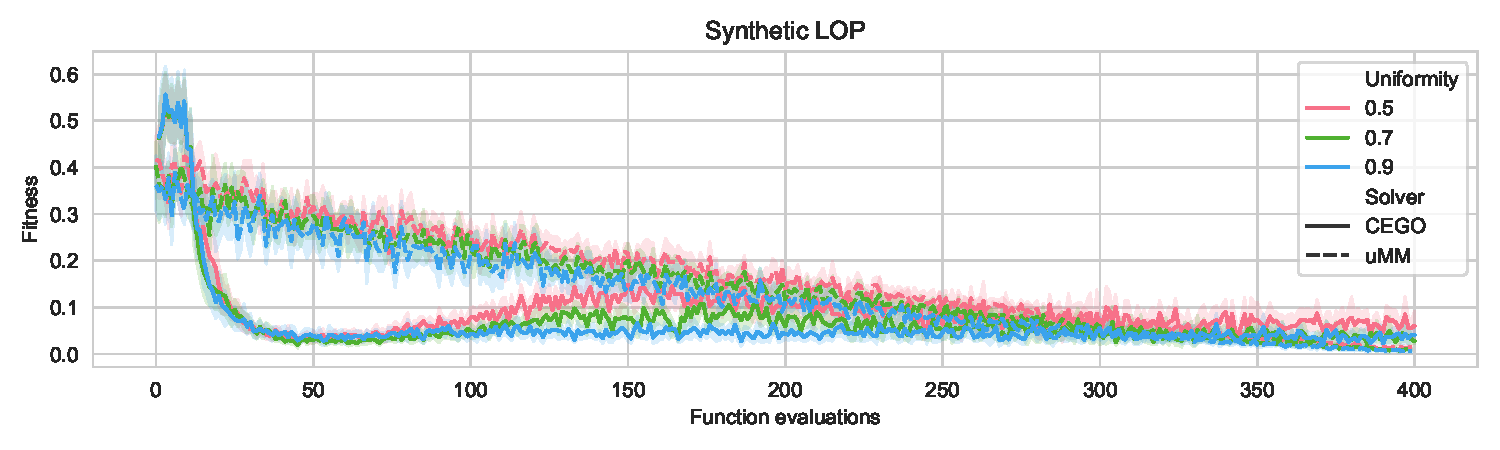
\includegraphics[width=\textwidth]{img/synthetic_LOP_combined}
  \caption{Mean fitness  (and standard deviation)  of each solution evaluated by each algorithm on LOP synthetic instances.\label{fig:lop_synth}}
\end{figure}

When we compare the behaviour of CEGO and uMM on synthetic LOP instances
(Fig.~\ref{fig:lop_synth}), we observe a clear pattern independently of the
uniformity of the instances. In particular, CEGO starts with a random sampling
of X solutions, with are quite poor as expected, followed by building and
updating the Kriging model based new evaluations, which leads to an impressive
improvement in less than 50 evaluations. However, progress is more or less
halted at this point and the model seems to have trouble generating better
solutions. Lower uniformity values (e.g., $\mu=5$) show worsening evaluations
despite the increase in solutions used to build the model. In summary, the
Kriging model clearly helps CEGO to quickly identify good solutions in very few
evaluations. However, for some reason, CEGO is not able to further improve
those solutions given more data. This may due to the model not being able to
produce accurate predictions or the underlying optimizer not being able to find
improved solutions using the model.\MANUEL{perhaps we should measure the
  prediction error and see if it grows or decreases. That would answer this
  question.}


On the other hand, uMM converges much more slowly than CEGO, only reaching the
same fitness values around evaluation 250. Yet, uMM is able to keep the rate of
improvement and completely overtake CEGO around evaluation 350. As in the case
of CEGO, lower uniformity values lead to worse performance, although the
difference is much smaller for uMM than it was for CEGO.\MANUEL{If there is anything else we can say here, please go ahead and say it}


\newcommand{\supplement}{\citep{Supplementary}}


%: LOP reales: he puesto 3 de diferentes tamanos. Me ha parecido interesante que, a pesar de que CEGO parece que va mejor, esta diferencia se va reduciendo segun se aumenta el tamano del problema (que se puede ver en el nombre del problema y en el títutlo de la gráfica)
\begin{figure}[tb]
  \centering%
  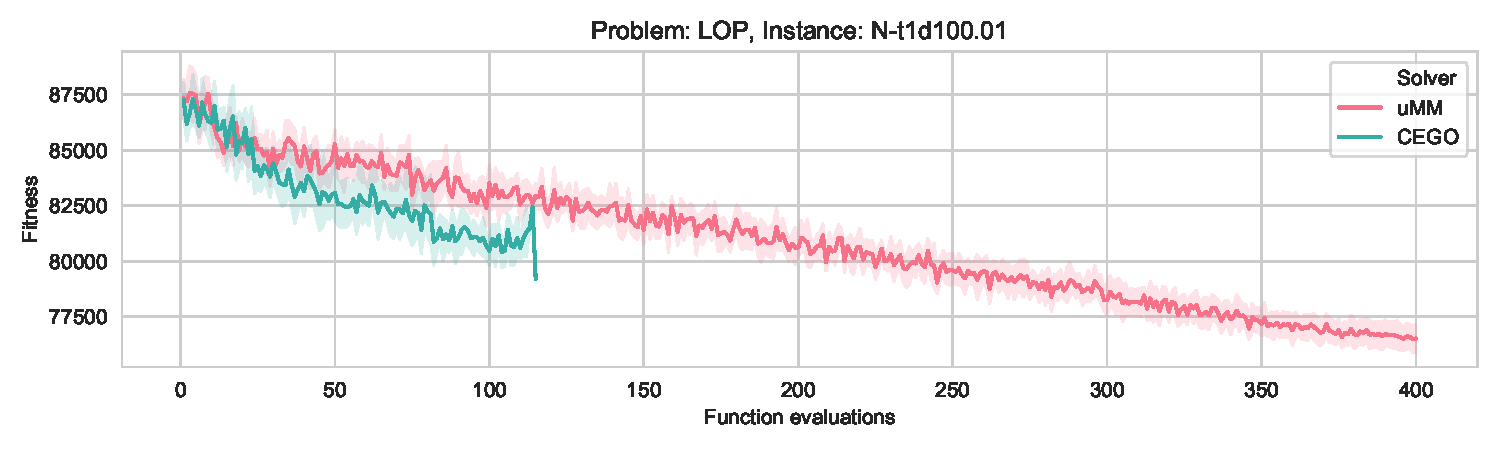
\includegraphics[width=\textwidth]{img/fitness_real_lop_RandA1_N-t1d100_01}\\
  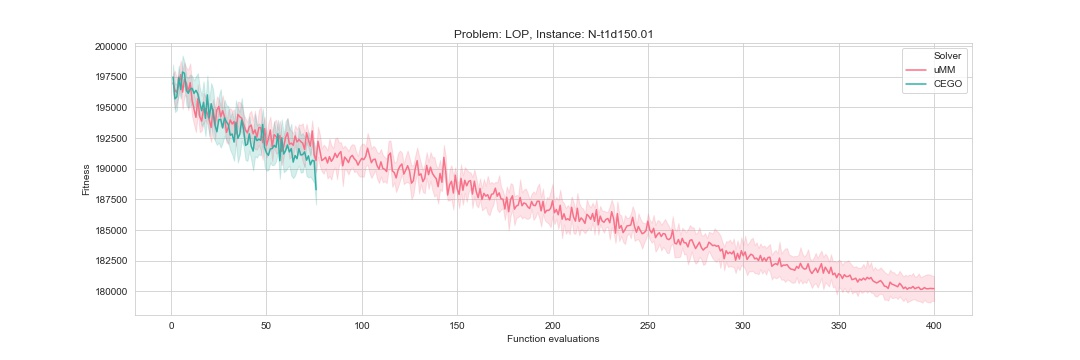
\includegraphics[width=\textwidth]{img/fitness_real_lop_RandA1_N-t1d150_01}\\
  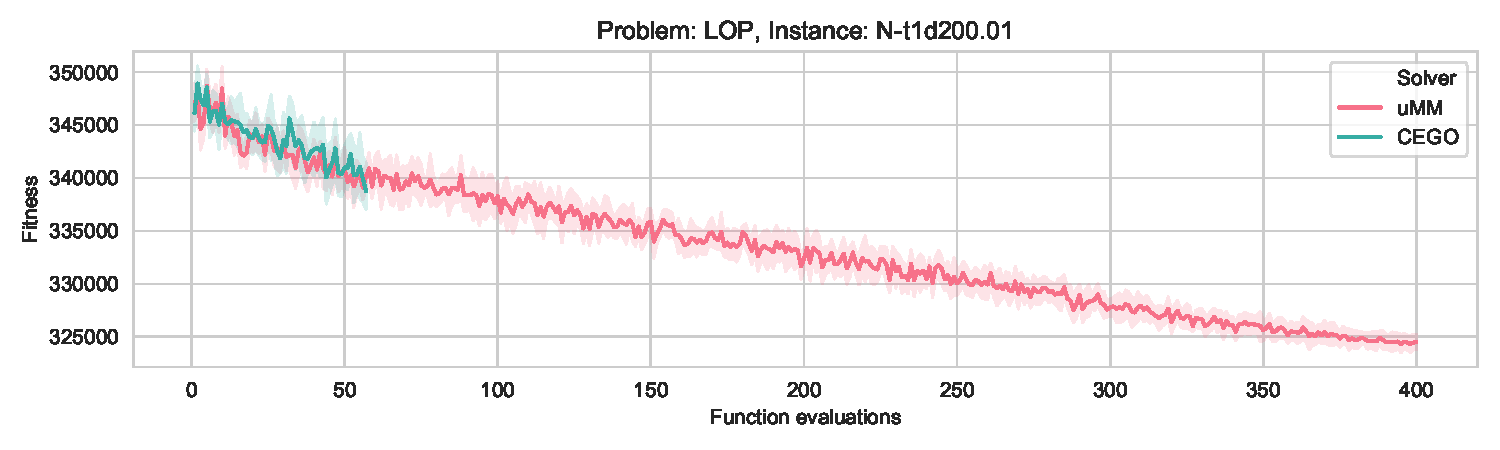
\includegraphics[width=\textwidth]{img/fitness_real_lop_RandA1_N-t1d200_01}\\
    \caption{Mean fitness  (and standard deviation)  of each solution evaluated by each algorithm on three instances from LOPLIB.\label{fig:loplib}}
  \end{figure}


Results are quite different on the 
%The fast initial convergence of CEGO for synthetic LOP instances does not seem
%to translate to the
instances available in LOPLIB~\citep{}. We show in
Fig.~\ref{fig:loplib} three examples with different permutation size, however,
the results are consistent for other LOPLIB instances (complete results
available as supplementary material \supplement). Due to extremely long
runtimes of CEGO and constraints in our computing system, we set a maximum
wall-clock time of 3 days for each run of CEGO. On these instances, the
behaviour of CEGO and uMM is much more similar (at least up to the termination
point of CEGO). It appears that our synthetic LOP instances have a fitness
landscape that is very amenable to CEGO's Kriging model, whereas the LOPLIB
instances do not present such landscape. Comparing CEGO and uMM results, the
differences get smaller, in favour of uMM, with larger instance size. Our
conjecture is that building an accurate Bayesian model and searching for good
solutions on it becomes harder for larger fitness landscapes.
\EKHINE{Parece que el paper va del CEGO en vez del UMM :p. Yo diría que tanto UMM como CEGO encuentran soluciones que mejoran según avanzan, pero con diferencias de comportamiento: (1) las los optimos de UMM son '3 veces mejor', y esto yo creo que es importante, aunque en gran parte se debe a que (2) UMM hace 400 ejecuciones en 3, 6 y 11 horas y CEGO entre 50 y 130 en 5 dias (3) cego empeora segun n aumenta (y n=200 tampoco es enorme)}
\MANUEL{Eso es porque puedo interpretar los resultados de CEGO mejor que los de UMM. Si crees que hay alguna interpretación o conjetura sobre UMM que podemos mencionar aquí, sería bueno mencionarla.}
\MANUEL{Prefiero dejar el comentario sobre las mejores soluciones encontradas y el tiempo requerido para cuando hable de la tabla, así se puede ver todo junto}

In the case of the PFSP, none of the algorithms are able to achieve a progress
better than a random search would, as illustrated by the results
(Fig.~\ref{fig:rec05}) obtained on \texttt{rec05}, which is the smallest PFSP
instance considered here. The lack of any apparent convergence suggests that
the models (both Bayesian and probabilistic) are not learning anything about
the fitness landscape. Results for larger PFSP corroborate this conclusions
(\supplement). Although previous studies~\citep{ZaeStoBar2014:ppsn} concluded
that other distance measures are more suited than Kendall's-$\tau$ distance for
the PFSP, the reported fitness differences between various distance metrics are
small, hence, we conjecture that the same behaviour will be observed with other
distance metrics.
  

\begin{figure}[tb]
  \centering%
  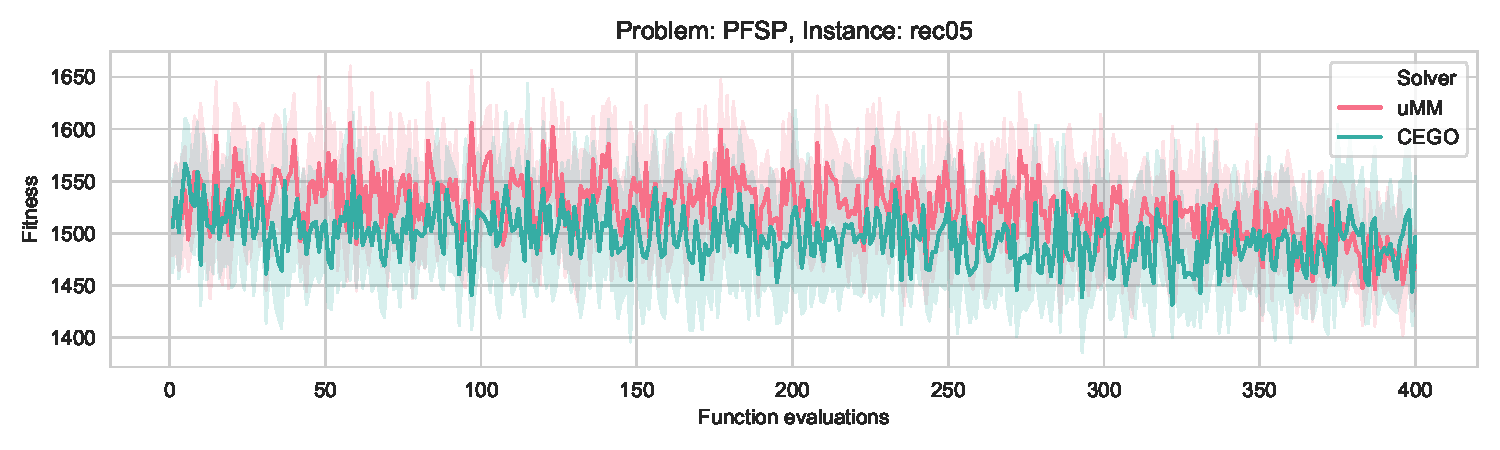
\includegraphics[width=\textwidth]{img/fitness_real_pfsp_rec05_txt}
  \caption{Mean fitness  (and standard deviation)  of each solution evaluated by each algorithm on the PFSP instance \texttt{rec05}.\label{fig:rec05}}
\end{figure}

The situation is very similar for the QAP, where both algorithms show the same
behaviour as in the PFSP for all instances tested, except for
\texttt{kra32}. As shown in Fig~\ref{fig:kra32}, in this instance both
algorithms are able to improve over the number of evaluations, although not
with ease. As in the synthetic LOP instances, we again observe that CEGO does
improve faster than UMM initially, yet, around evaluation 250, it appears to
get stuck and around evaluation 300, UMM overtakes it. We believe the reason is
the same as before, that is, the model is not able to adequately reflect the
ruggedness of the actual landscape and, hence, the best solutions found by the
GA searching the model are not improved solutions for the actual problem. Interestingly, \texttt{kra32} is rectangular
whereas \texttt{tho32} contains rectangular distances and \texttt{nug12} and \texttt{nug30} contain Manhattan distances of rectangular grids.\MANUEL{so they all have the same distance type!!! What is the difference then? Ask Thomas?}

\begin{figure}
  \centering%
  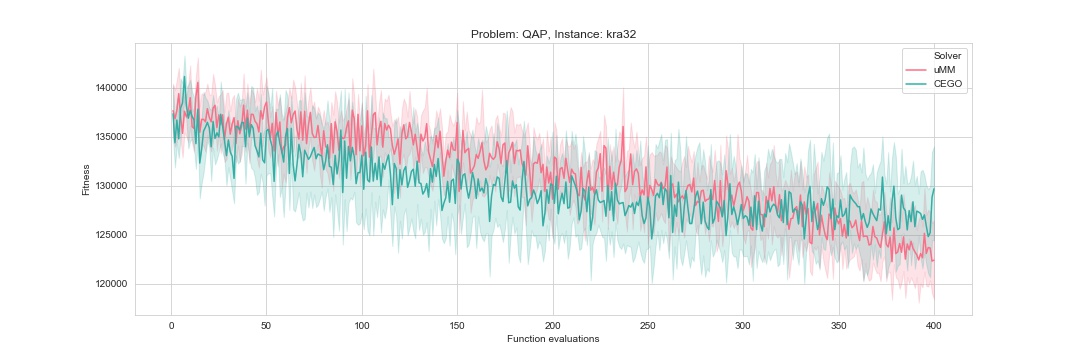
\includegraphics[width=\textwidth]{img/fitness_real_qap_kra32_dat}
    \caption{Mean fitness  (and standard deviation)  of each solution evaluated by each algorithm on the QAP instance \texttt{kra32}.\label{fig:kra32}}
\end{figure}

Table~\ref{tab:results} shows overall results over all instances evaluated (excluding the synthetic LOP instances). In particular, the mean fitness (and standard deviation) of the best solution found at the end of each run,
\MANUEL{is the CI for CEGO $-$ UMM or UMM $-$ CEGO? I would prefer}
In terms of best fitness achieved on each run, and taking into account the
random behaviour observed in some instances and discussed above,



   \newcommand{\mcolc}[2]{\multicolumn{#1}{c}{\bf #2}}
\begin{table}[tb]
 \caption{Mean fitness (and standard deviation) of the best solution found at the end of each run, over 10 independent runs for each problem instance. The 95\% confidence interval corresponds to the two independent samples t-test on the mean of the difference between the fitness of UMM minus the one of CEGO. Mean runtime is measured in hours. If a run went over 72 hours, of  CEGO was not able to reach 400 function evaluations (FEs) in 72 hours, it was terminated earlier. This was the case for all LOP instances shown.\label{tab:results}}
 \resizebox{\textwidth}{!}{%
\begin{tabular}{*{6}{r}rl*{3}{r}}
 \toprule
            &                  & \mcolc{4}{Mean fitness (sd)} & \mcolc{2}{\multirow[b]{2.45}{*}{\shortstack{95\% CI for the\\mean difference}}} & \bf \multirow[b]{2.45}{*}{\shortstack{Mean FE\\CEGO}} & \mcolc{2}{Mean runtime} \\\cmidrule{3-6}\cmidrule(lr){10-11}
\bf Problem & \bf     Instance & \mcolc{2}{CEGO} & \mcolc{2}{UMM}   &                         &            & \bf & \bf CEGO       & \bf UMM                       \\\midrule
    LOP     & N-t1d100.01      & 78696.6                 & (811.4)    & 76119.6   & (915.4)                & $[$1763.5,    & 3390.5$]$     & 111.8& 72.5 & 3.2  \\
    LOP     & N-t1d100.02      & 79686.5                 & (367.9)    & 76827.7   & (891.0)                & $[$2194.5,    & 3523.1$]$     & 110.7& 72.9 & 3.2  \\
    LOP     & N-t1d150.01      & 187605.5                & (1906.9)   & 179508.3  & (1647.9)               & $[$6420.3,    & 9774.1$]$     & 73.9 & 72.7 & 6.5  \\
    LOP     & N-t1d150.02      & 184320.9                & (973.5)    & 177592.8  & (1196.2)               & $[$5700.5,    & 7755.7$]$     & 74.1 & 73.2 & 6.5  \\
    LOP     & N-t1d200.01      & 335391.1                & (2289.0)   & 323513.6  & (1371.2)               & $[$10076.1,   & 13678.9$]$    & 55.6 & 73.2 & 10.7 \\
    LOP     & N-t1d200.02      & 333149.5                & (2497.2)   & 319675.8  & (2242.6)               & $[$11242.0,   & 15705.4$]$    & 56.5 & 73.7 & 10.6 \\
    LOP     & N-t2d150.01      & 24682.7                 & (976.6)    & 15297.7   & (563.5)                & $[$8622.2,    & 10147.8$]$    & 74.6 & 72.9 & 7.0  \\
    LOP     & N-t2d150.02      & 24250.8                 & (1354.9)   & 14724.9   & (667.5)                & $[$8495.1,    & 10556.7$]$    & 74.8 & 72.8 & 7.1  \\
    LOP     & N-t2d200.01      & 57098.6                 & (4452.8)   & 33465.2   & (2001.0)               & $[$20284.5,   & 26982.3$]$    & 56.3 & 73.3 & 11.2 \\
    LOP     & N-t2d200.02      & 54895.6                 & (4589.7)   & 35901.8   & (2077.5)               & $[$15539.1,   & 22448.5$]$    & 55.6 & 73.5 & 11.2 \\
    LOP     & N-p50-01         & 21431.2                 & (299.5)    & 21027.6   & (711.8)                & $[$-128.1,    & 935.3$]$      & 219.9& 72.3 & 0.9  \\
    LOP     & N-p50-02         & 22021.1                 & (275.6)    & 21613.6   & (596.4)                & $[$-42.5,     & 857.5$]$      & 217.3& 72.3 & 0.9  \\
    LOP     & N-atp111         & 693.1                   & (10.3)     & 594.0     & (15.4)                 & $[$86.7,      & 111.5$]$      & 98.7 & 72.5 & 4.1  \\
    LOP     & N-atp134         & 880.5                   & (18.6)     & 756.3     & (21.3)                 & $[$105.4,     & 143.0$]$      & 83.0 & 72.8 & 5.7  \\
    LOP     & N-be75eec\_150   & 1666193.1               & (72310.8)  & 1415208.5 & (58593.5)              & $[$188960.6,  & 313008.6$]$   & 74.0 & 72.9 & 6.9  \\
    LOP     & N-be75eec\_250   & 5214413.0               & (166701.4) & 4431271.0 & (109756.7)             & $[$649040.8,  & 917243.2$]$   & 44.9 & 73.7 & 15.5 \\
    LOP     & N-be75np\_150    & 3742444.0               & (88500.2)  & 3204878.3 & (80704.1)              & $[$457944.2,  & 617187.2$]$   & 74.2 & 72.9 & 6.9  \\
    LOP     & N-be75np\_250    & 10887427.8              & (159642.5) & 9544754.9 & (260523.9)             & $[$1136635.8, & 1548710.0$]$  & 45.3 & 74.0 & 15.5 \\
   PFSP     & rec05.txt        & 1317.9                  & (25.1)     & 1330.7    & (17.9)                 & $[$-33.4,     & 7.8$]$        & 400.0& 38.9 & 0.1  \\
   PFSP     & rec13.txt        & 2128.2                  & (25.0)     & 2158.7    & (29.5)                 & $[$-56.2,     & -4.8$]$       & 400.0& 38.9 & 0.1  \\
   PFSP     & rec19.txt        & 2398.6                  & (19.8)     & 2405.1    & (12.6)                 & $[$-22.3,     & 9.3$]$        & 400.0& 82.1 & 0.3  \\
    QAP     & kra32.dat        & 115907.0                & (4663.4)   & 116320.0  & (4673.5)               & $[$-4799.3,   & 3973.3$]$     & 400.0& 95.8 & 0.3  \\
    QAP     & nug12.dat        & 624.2                   & (26.3)     & 660.4     & (17.3)                 & $[$-57.3,     & -15.1$]$      & 400.0& 14.8 & 0.0  \\
    QAP     & nug30.dat        & 7486.8                  & (40.4)     & 7474.0    & (83.9)                 & $[$-50.8,     & 76.4$]$       & 400.0& 84.3 & 0.3  \\
    QAP     & tho30.dat        & 192416.0                & (2584.2)   & 191482.0  & (4419.7)               & $[$-2527.0,   & 4395.0$]$     & 400.0& 85.1 & 0.3  \\
\bottomrule
\end{tabular}}
\end{table}




\section{Conclusions}

Bayesian optimization methods using a global GP model, such as CEGO, are known
to have trouble optimizing locally \citep{EriPeaGar2019scalable}. Our
intuition is that this problem becomes worse in rugged combinatorial
landscapes, where small steps may produce drastic changes.

Open questions:
\begin{itemize}
\item How difficult is to extend uMM to other distance metrics?
\item Can we plot the posterior probability of the optimal solution?
\end{itemize}

\paragraph*{Acknowledgements.}

Thanks to Hao Wang (Leiden University) for pointing us to the arguments of
\citet{EriPeaGar2019scalable}.




\renewcommand{\doi}[1]{doi:\hspace{.16667em plus .08333em}\discretionary{}{}{}\href{https://doi.org/#1}{\urlstyle{rm}\nolinkurl{#1}}}
\bibliographystyle{splncs04nat}
\bibliography{optbib/abbrev,optbib/authors,optbib/journals,optbib/biblio,optbib/crossref,./mendeley}

\end{document}

%%% Local Variables:
%%% mode: latex
%%% TeX-master: t
%%% End:
